\section{Security Framework Overview}

In this section, we begin by explaining the security policy model of
DASF that we designed. Afterward, we focus on
the architecture and implementation of the DASF prototype on Android.

\subsection{Security Model}

On an Android device, there are
a set of applications, $A := \left\{a_{1},a_{2},\ldots,a_{n}\right\}$.
Each application, $\forall a_{i} \in A$, where $1 \le i \le n$,
contains a set of permissions that the application requests,
$P_{a_{i}} := \left\{p_{1}, p_{2},\ldots,p_{m}\right\}$,
and a set of components,
$C_{a_{i}} := \left\{c_{1},c_{2},\ldots,c_{q}\right\}$.
Each application is either a system application, $S_{A}$,
or a third-party application, $T_{A}$, such that $S_{A}\subset A$, and $T_{A} \subset A$,
but $S_{A} \cap T_{A} = \left\{\right\}$.

\textbf{Dynamic Privilege Restriction Security Policy.}  A
permission, $p$, is restricted if the restricted permission, denoted
as $R\left(p\right)$, is imposed
by a specific application $a_{i}$.
%such that $a_{j} \in A$ and $1 \le j \le m$.  
In Android, permissions are granted at the granularity
of the entire application.  If the permissions of a specific
application, $a_i$, is granted, its corresponding components,
$C_{a_i}$ are allowed to be launched. Obviously, for any application
that can successfully run, each of its components has to have the
permission to be launched. We use $L(C_{a_i})$ to
denote the launching of $a_i$'s components: $c_1, c_2,...,c_q$.
%
%Since permissions are granted at the granularity
%of the entire application rather than at the granularity of its individual
%components, the application's components that are permitted
%to be launched is denoted as $L\left(C_{a_{i}}\right)$. This means,
%$\forall c_{k} \in C_{a_{i}} : L\left(c_{k}\right)$ such that 
%$1 \le k \le o$.  
Furthermore, we denote killing the process
that an application, $a_{i}$, is running under as $K(a_{i})$.

Therefore, the security policy for an application is a procedure of
imposing the restricted permissions which determine whether or not the
application and its components can be launched. Given an application
$a_i$, its components launching, $L(C_{a_i})$, will be
successful as long as one the security policy satisfy any one of the
following conditions:

\[\left\{
\begin{array}{l}
a_i \in S_A\\
a_i \in T_A \wedge R\left(p\right) \wedge p \in P_{a_{i}} \wedge
a_i = a_j\\
a_i \in T_{A} \wedge \lnot R\left(p\right) \wedge p \in P_{a_{i}}.\\
\end{array}
\right.
\]


%for starting an application, $a_{i}$,
%and it's components, $C_{a_{i}}$, is defined as follows.

%$a_{i} \in S_{A} \to L\left(C_{a_{i}}\right)$

%$a_{i} \in T_{A} \wedge R\left(p\right) \wedge p \in P_{a_{i}} \wedge a_{i} = a_{j} \to L\left(C_{a_{i}}\right)$

%$a_{i} \in T_{A} \wedge \lnot R\left(p\right) \wedge p \in P_{a_{i}} \to L\left(C_{a_{i}}\right)$

\begin{comment}
$a_{i} \in T_{A} \wedge R\left(p\right) \wedge p \in P_{a_{i}} \wedge a_{i} \neq a_{j} \to \lnot L\left(C_{a_{i}}\right)$
\end{comment}
More significantly, DASF is able to impose the
policy on application that are already running when a permission is
dynamically restricted for a security purpose.  In that case, any
running application $a_i$ with the following updated policy:
\[\left.
\begin{array}{l}
(a_{i} \in T_{A}) \wedge R\left(p\right) \wedge (p \in P_{a_{i}})\\
\end{array}
\right.
\]
will lead to $K(a_i)$, i.e., be terminated.  And the running
application status with the following
new policy:
\[\left \{
\begin{array}{l}
a_{i} \in S_{A}\\
a_{i} \in T_{A} \wedge \lnot R\left(p\right) \wedge p \in P_{a_{i}} \wedge a_{i} = a_{j}\\
\end{array}
\right.
\]
will become $\lnot K(a_i)$, i.e., not be affected.
%Moreover, the security policy imposed on applications that are 
%already running when a permission is dynamically restricted
%is defined as follows.

%$a_{i} \in S_{A} \to \lnot K\left(a_{i}\right)$

%$a_{i} \in T_{A} \wedge \lnot R\left(p\right) \wedge p \in P_{a_{i}} \wedge a_{i} = a_{j} \to \lnot K\left(a_{i}\right)$


%$a_{i} \in T_{A} \wedge R\left(p\right) \wedge p \in P_{a_{i}} \to K\left(a_{i}\right)$

In other words, an application's components are always allowed to
start if they belong to a system application.  Moreover, system
applications are never forcibly closed if a permission is dynamically
restricted.  If the application is a third-party application, however,
the following policies are enforced. First, a third-party
application's components are not permitted to start if the application
requests a permission that is currently restricted and the application
is not the one that imposed the permission restriction.  Second, a
third-party application's components are permitted to start if the
application does not request any permissions that are currently
restricted or if the permission is currently restricted and the
application is the one that imposed the permission restriction.
Furthermore, if a permission is dynamically restricted and a
third-party application that is currently running has requested that
permission and was not the application that imposed the permission
restriction, the application will be forcibly closed.

Since DASF provides support for third-party
applications to programmatically restrict permissions, the
application, $a_{i}$, must define a set of permissions that it is
permitted to restrict, $X_{a_i} := {p_1, p_2,\ldots,p_m}$,
during the application's installation and approved by the user to prevent
the abuse of dynamic permission restrictions.  Thus, a third-party application,
$a_{i}$, is allowed to restrict a permission, $p$, if $p \in X_{a_{i}}$.

\textbf{Security Policies on Sensitive Data.}
A mobile device contains a set of data (e.g., strings, integers, arrays,
etc.) in RAM, $\left\{d_{1},d_{2},\ldots,d_{n}\right\}$,
each of which has its corresponding sensitivity level. In our
framework, we use a privacy tag, $T(d_i)$, with the possible values of
$\left\{t_{1},t_{2},\ldots,t_{m}\right\}$, to represent data $d_i$'s
sensitivity level.
%$\left\{t_{1},t_{2},\ldots,t_{m}\right\}$, to represent a variety of 
%sensitivity levels.  
%privacy tag: $T(d_i)$, where $1\leq i\leq n$. 
%Since we utilize the dynamic taint tracking system provided
%by TaintDroid, each element in the set of data also includes
%a privacy tag, $T\left(d_{i}\right)$, which denotes the data's sensitivity level
%that comes from the set of possible privacy tags,
%$\left\{t_{1},t_{2},\ldots,t_{m}\right\}$.
%%
%
%Thus, we denote the set of data in the Java stack as a set
Thus, we can denote the data set as a set containing a privacy tag and
the data:
%containing a privacy tag and the data,
$D := \left\{\left\{d_{1}, T\left(d_{1}\right)\right\},\left\{d_{2},T\left(d_{2}\right)\right\},\ldots,\left\{d_{n},T\left(d_{n}\right)\right\}\right\}$.

It is possible for two pieces of data, $d_{j}$, $d_{k}$, where $1 \le
j \le n$ and $1 \le k \le n$,  with different privacy tags
to be combined (e.g., concatenating two strings with different
sensitivity levels).  The general propagation rules of the
privacy tags are as follows when data with two different privacy tags
are combined, $d_{j} + d_{k}$.

$T(d_{j}) \ge T(d_{k}) \to T(d_{j}+d_{k}) = T(d_{j})$

$T(d_{j}) < T(d_{k}) \to T(d_{j}+d_{k}) = T(d_{k})$

These propagation rules ensure that when two pieces of
data are combined, the highest sensitivity level is propagated
to the combined data.   This means that if the sensitivity
level of $d_{j}$ is greater than or equal to the sensitivity
level of $d_{k}$, the combined data has the sensitivity level
of $d_{j}$.  Further, if the sensitivity level of $d_{j}$ is
less than the sensitivity level of $d_{k}$, the combined data
has the sensitivity level of $d_{k}$.

We define two operations on the data that our security policy
must handle.  First, $W(d_{j})$, denotes writing the data to
flash memory (e.g., to a file or an SQLite database). Second,
$F(d_{j})$ denotes forwarding the data from the device
(e.g., through a socket, bluetooth socket, SMS, and MMS).
Furthermore, data, $d_{j}$, that can not be forwarded from the
device nor written to flash memory is denoted as $FW\left(d_{j}\right)$.
The operations that are permitted on the data are determined by the
data's privacy tag.  The privacy tag, $t_{m}$, denotes
that $T(d_{j}) = t_{m} \to \lnot FW\left(d_{j}\right)$. The privacy tag,
$t_{m-1}$, denotes $T(d_{j}) = t_{m-1}\lnot W\left(d_{j}\right)$.  Finally,
the privacy tag, $t_{m-2}$, denotes 
$T(d_{j}) = t_{m-2} \to \lnot F\left(d_{j}\right)$.  Furthermore, we reserve
the privacy tag, $t_{m-3}$ to denote sensitive information that have
no security policies enforced by the system.

To ensure that the security policies are enforced correctly when
combining two pieces of data with different sensitivity levels,
the propagation rules of the data's sensitivity levels must
include an escalation of sensitivity levels.  For example, if
data with the privacy tag $t_{m-1}$ is combined with data with
the privacy tag $t_{m-2}$, the combined data should have the
privacy tag $t_{m}$ rather than $t_{m-1}$.  Thus, the propagation
of privacy tags are adjusted as follows when data is combined,
$d_{j} + d_{k}$.

$T\left(d_{j}\right) = t_{m-1} \wedge T\left(d_{k}\right) = t_{m-2} \to T\left(d_{j}+d_{k}\right) = t_{m}$

This propagation rules ensures that if data that is restricted from
being forwarded from the device is combined with data the is restricted
from being written to flash memory, the combined data will be restricted
from being written to the flash memory and forwarded from the device.

\textbf{Application-Layer Message Protocol.}   DASF
also includes an application-layer message protocol
that allows a server to dynamically enforce privilege restrictions
on the device and enforce the previously mentioned security policies
on data that is sent to the device.  The message
protocol assumes that it is built over an SSL connection to ensure
a secure communication channel between the client (e.g., mobile
device) and the server.

The message protocol consists of applications sending a request to
the server (e.g., requesting data) and the server responding back
to the request (e.g., sending the data).  The message protocol
allows the server to impose a sensitivity level on the data in
its response, and thus, impose a security policy on the data that
it sends to the client.  We call the server responding to the
client's request for data as a \textit{data message}.
The header of the \textit{data message} denotes the type of message,
sensitivity level, and the length of the payload.  The contents of a
\textit{data message} is shown in Fig.~\ref{fig:datamessage}.

\begin{figure}[ht]
\centering
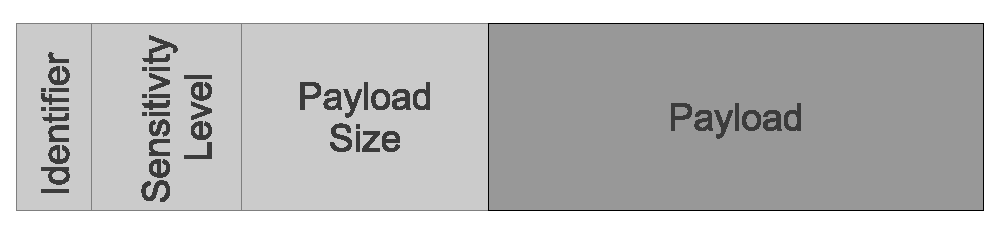
\psfig{file=data_message.eps, width=2.5in}
\caption{Data Message}
\label{fig:datamessage}
\end{figure}

\vspace{-3mm}

When an application requests data from the server, the server
responds back to the client with
$data\_message\left(\left\{sensitivity\_level, response\right\}\right)$.
The system extracts sensitivity level and applies that sensitivity level
to the response before passing it to the application.  The sensitivity
level, $s$, corresponds to one of the four privacy tags that we previously defined.
Thus,  $s \in \left\{t_{m-3}, t_{m-2}, t_{m-1}, t_{m}\right\}$.

The server can also dynamically impose any privilege restrictions on
the device without asking the user for permission.  To prevent the
abuse of server-imposed privilege restrictions, the application must
be declared as a \textit{medical application} during its installation
and the system insures that the client application connects to the
organization's trusted server.  The server may dynamically impose
privilege restrictions, or unrestricted previously imposed privilege
restrictions, on the device by prepending a
\textit{privilege control message} to the \textit{data message}.
Furthermore, the payload of the \textit{privilege control message} must be
encrypted using a one-time key to prevent applications from abusing
this functionality.  The payload must be encrypted with a one-time
key so that DASF can verify that the policy
originated from the server and to prevent replay attacks.  Our
security framework fetches the initial secret key from the server
when the device is first booted.

The payload of the \textit{privilege control message} contains a list
of privilege restrictions, privilege unrestrictions, and a new secret
key.  The entire payload is encrypted using the previous key,
$E\left(key, payload\right)$.  The header of the \textit{privilege control
 message} contains the type of message, a flag denoting that a data message
is appended, and the length of the payload. The contents of 
a \textit{privilege control message} is shown in
Fig.~\ref{fig:privilegemessage}.  When the system receives a
\textit{privilege control message}, it passes the payload to DASF.
If the security framework successfully decrypts
the payload, $D\left(key, payload\right)$, the set of permission restrictions
and unrestrictions are imposed and the secret key is updated.

\begin{figure}[ht]
\centering
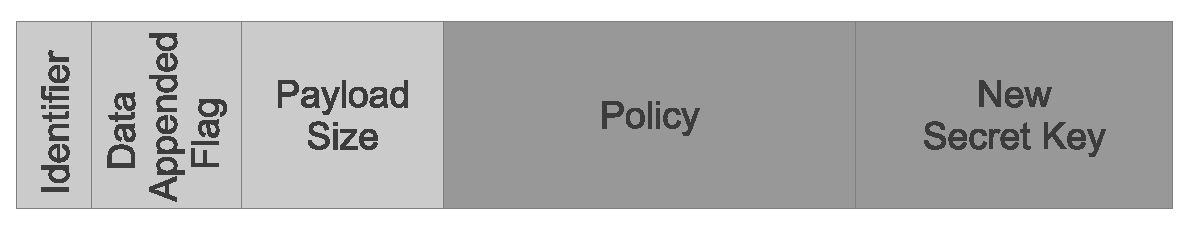
\psfig{file=policy_message.eps, width=2.5in}
\caption{Privilege Control Message}
\label{fig:privilegemessage}
\end{figure}

\vspace{-5mm}
\subsection{Prototype Implementation}

We implemented the prototype of DASF on Android 4.1.1
(\textit{Jelly Bean}) and TaintDroid.  We have also implemented a
server program that utilizes our message protocol to transfer data
and dynamic privilege restrictions and unrestrictions to DASF
and applications running on our prototype.  We assume
that DASF utilizes the CleanOS extension of TaintDroid, which
provides a mechanism for revoking access to tainted data. However, our prototype
is actually directly implemented over the TaintDroid platform because
the source code for the CleanOS project was not available.  Regardless
of that fact, our security model is designed to be easily integrated into
the CleanOS architecture to take advantage of the data revocation
mechanism that it offers.

Specifically, the four sensitivity levels that our security model defines to
enforce security policies on sensitive can can be defined as the
highest sensitivity level of secure data objects on CleanOS.  Further,
CleanOS' propagation logic would need to be modified to handle
the escalating of sensitivity levels that correlate to security policies
when combining data with different sensitivity levels as mentioned in
our security model.  Also, the organization that sends the sensitive
data to the device would need to control CleanOS' cloud service that is
used for revoking sensitive data.  However, since we implement our prototype
directly over TaintDroid, we emulate the sensitivity levels mentioned above
by defining four custom privacy tags and enforce the system restrictions based
off of those tags.

The architecture of the prototype of DASF consists
of three modifications to the Android platform and TaintDroid.  
First, we defined the four privacy tags mentioned in the previous section
and placed hooks in the Java libraries to enforce the security policies
on sensitive data.  Second, we implemented a system service that is
responsible for managing the dynamic system-wide privilege restrictions
and placed hooks in the Android framework libraries to enforce the privilege
restrictions.  Third, we implemented the message protocol in the system
to tag sensitive data that is received from the server and modified the
Java libraries to force \textit{medical applications} to use our message
protocol.

\textbf{Restriction Policy Manifest File.}  For applications to utilize
DASFk, the application must include a special manifest
file that is parsed during the application's installation.  As stated
in our security model, DASF allows applications to
dynamically enforce system-wide permission restrictions that may be
programmatically set in an application's code or by receiving messages
from the trusted server using DASF's message protocol. In order
to prevent malicious applications from abusing the system-wide permission
restrictions that are imposed by the server, DASF limits their
use to applications that are declared as a \textit{medical applications} in
their \textit{restriction\_policy.xml} file.  Furthermore, we
force all applications that are declared as \textit{medical applications}
to use our message protocol and communicate directly with the trusted
server.  All system-wide permission restrictions that are set
programmatically in an application must be declared at the time
of the application's installation and approved by the user to
prevent application programmers from maliciously imposing restrictions
on the device. However, the trusted server can dynamically restrict
any permission on the device at runtime without the user's permission
to allow organizations to dictate the security policies on the device
on-the-fly. 

The \textit{restriction\_policy.xml} manifest file is an XML file
that must be included in the \textit{/assets/} directory in the
application's APK in order for an application to utilize DASF.
The \textit{restriction\_policy.xml} file is responsible for declaring the
system-wide permission restrictions that may be set programmatically by
the application and declaring the application as a \textit{medical 
application} to allow for system-wide permission restrictions
imposed by the server. An example \textit{restriction\_policy.xml} file
that allows the trusted server to dynamically restrict any permissions
on the device and allows the application to programmatically restrict
the access to the microphone and camera is shown in
Fig.~\ref{fig:policy}.  

\begin{figure}[ht]
\centering
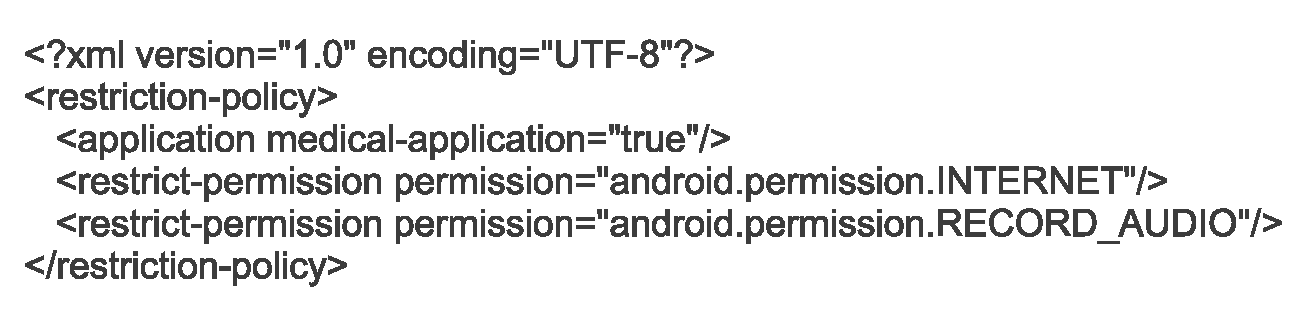
\psfig{file=restriction_policy.eps,width=3.0in}
\caption{An example of a policy restriction file.}
\label{fig:policy}
\end{figure}
%\vspace{-8mm}

\textbf{Dynamic Privilege Restrictions Implementation.}  We
implemented a system service, named the \textit{Privilege Restriction
 Service}, that is responsible for enforcing and imposing the
dynamic system-wide privilege restrictions on applications.  
The \textit{Privilege Restriction Service} contains four
hash maps to store necessary information that DASF needs
to enforce privilege restrictions on applications.  The four hash maps store
the following information.

\begin{itemize}
\item \textit{Medical application hash map:} Stores packages that are tagged
  as medical applications.
\item \textit{Requested permissions hash map:} Stores all of the \textit{uses-permissions}
  that an application requests.
\item \textit{Restriction policy hash map:} Stores the privileges that an application can
  programmatically restrict.
\item \textit{Restricted privileges hash map:} Stores the system-wide permission
  restrictions currently imposed on applications.
\end{itemize}

We decided to store the package information in RAM rather than on flash
memory in order to prevent unauthorized modification of our
framework's data (e.g., pulling a file via a USB connection,
changing the contents and then pushing it back to the device).
Furthermore, DASF can repopulate the hash maps if the device
is shutdown since Android reparses all of the installed packages during the
boot process, which makes main memory the ideal location to store our
framework's data.  Moreover, the entries that are enforced by the
server in the \textit{restriction policy hash map} can be
restored to its previous state since our \textit{Privilege Restriction Service}
communicates with the trusted server during the boot process.  The \textit{Privilege Restriction Service} is started by Android's \textit{Service Manager} when the
device boots.  When the \textit{Privilege Restriction service} starts, it
communicates with the server to fetch the secret key needed to decrypt
security policies received from the server.  

We placed a hook in Android's \textit{Package Parser} to parse the
\textit{restriction\_policy.xml} manifest file.  If the application
is being installed,
the user is notified if the APK's restriction policy file includes the
\textit{medical application} tag and the restricted permissions policy
that it declares. For the application to continue installation, the
user must approve the policies that are declared in the restriction
policy file.  If the user approves the policies, a hook in the
\textit{Package Manager Service} invokes the \textit{Privilege Restriction
 Service} to add the \textit{uses-permissions} that an application requests
in its manifest file to the \textit{requested permissions hash map}.
Furthermore, the hook in the \textit{Package Manager Service} also
invokes the \textit{Privilege Restriction Service} to populate the
\textit{medical applications hash map} and the
\textit{restriction policy hash map} if the application included
the \textit{restriction\_policy.xml} manifest file.  We have
also restricted applications that are declared as
\textit{medical applications} from sharing a UID to ensure
that they run in their own isolated process and are the only application
that may access their application's directory and files.  Medical
applications must have a unique UID because a developer that creates
a medical application could maliciously create a different application
signed with the same developer signature to access the sensitive files
of the medical application.

We have provided an \textit{Privilege Restriction} class in the
\textit{android.} package that allows applications to programmatically
enforce a privilege restriction or unrestrict a previously restricted
permission.  The application can call the \textit{restrictPermission()}
method with the permission name as the argument of the method to restrict
a permission.  The \textit{restrictPermission()} method invokes
the \textit{Privilege Restriction Service} to check whether the
application that called the method has requested to restricted the permission
by checking the \textit{restriction policy hash map}.  If the permission
is in the \textit{restriction policy hash map} under the calling application's
entry, the permission restriction is imposed by adding an entry
to the \textit{restricted privileges hash map} and all currently running
applications that request that permission are closed.  Furthermore,
an application may unrestrict a previously imposed permission restriction
by calling the \textit{unrestrictPermission()} method with the permission
name as the argument of the method.  The \textit{unrestrictPermission()}
method invokes the \textit{Privilege Restriction Service} to ensure
that the application attempting the unrestrict the permission was
the application that imposed the restriction.  If the application's
UID matches the UID of the application that imposed the restriction,
the permission is unrestricted by removing the entry from the
\textit{restricted permissions hash map}.

We have placed hooks in the \textit{Activity Manager Service} so when 
an application's component (e.g., activities, services, broadcast receivers,
or content providers) is attempting to start, our \textit{Privilege Restriction
 Service} is called to enforce the security policies for starting applications
as defined in our security model.

\textbf{Sensitive Data Security Policies Implementation.}  Our
security framework allows an application developer to programmatically
classify the sensitivity level of data and also allows a server
to classify the sensitivity level of data that it sends to the device.
An application developer can programmatically classify data by calling
methods in the \textit{Data Classification} class that DASF
provides. For example, an application developer can prevent a string
containing PHI data from being written to the disk by calling the
\textit{preventDiskWrite()} method with the string as the argument.
The \textit{Data Classification} class also provides the following
methods, \textit{preventForwarding()} and
\textit{preventDiskWriteAndForwarding()} to enforce the
security policies on data as discussed in our security model.
These methods add the security policy's corresponding
privacy tag to the data.

We have placed hooks in the Android system to enforce the security
policies imposed on the sensitive data.  To prevent data
from being written to flash memory, we have placed a hook in the \textit{Posix}
class to enforce restrictions on data that is written to a file and the
\textit{SQLite} library to enforce restrictions on data that is
written to an SQLite database through insert and update statements.
These hooks check the privacy tag of the data attempted to be written
to flash memory and blocks writing the data if the privacy tag matches
the tags that prevent disk writes.  We assume that the
CleanOS SQLite patch for retaining privacy tags on retrievals
from the database is implemented to ensure correct propagation
of the privacy tags on individual entries.  To prevent data from
being forwarded from the device, we have placed hooks in the \textit{Posix}
class, the \textit{BluetoothSocket} class, and the \textit{SmsManager}
class to enforce whether PHI data is permitted to be sent over
a socket, a bluetooth connection, or through an SMS message.
These hooks check the privacy tag of the data attempted to be forwarded
from the device and blocks forwarding the data if the privacy tag matches
the tags that prevent forwarding data.

\textbf{Message Protocol Implementation.} As stated in our
security model, our message protocol consists of two different
types of messages.  First, the \textit{data message} is
used by the server to send data and the data's corresponding
sensitivity level to a medical application.  Second, the
server may prepend a \textit{permission control message} to a
\textit{data message} to impose system-level permission
restrictions, or unrestrictions, on the device.

Whenever a medical application requests data from the server
the server sends the requested data back to the application
as the payload of a \textit{data message}.  The \textit{data message}
contains a 4-byte header and a payload.  The header of the
\textit{data message} contains 1-bit to identify the type of
message, 2-bits to identify the sensitivity level that the server
imposes on the payload, and  29-bits for the length of the payload.
Thus, the server can transmit $2^{29}$ bytes of data in
one \textit{data message}.  However, if the server needs to transmit
more than $2^{29}$ bytes of data, it can break the response up
into multiple \textit{data messages}.

Furthermore, the server may also prepend a \textit{permission
 control message} to the \textit{data message}.  The
\textit{permission control message} contains a 2-byte header.
The header of the \textit{permission control message} contains
1-bit to identify the type of the message, 1-bit to denote
that a \textit{data message} is appended, and 14-bits for
the length of the payload.  Therefore, the server can
transmit $2^{14}$ bytes of permission restrictions and
permission unrestrictions in one \textit{permission control
 message}.

To force \textit{medical applications} to communicate with
the trusted server, we placed a hook in the \textit{Posix} class
to invoke our \textit{Privilege Restriction Service} to
determine whether the application is a \textit{medical application}
by checking whether or not the application's UID is in the
\textit{medical application hash map}.  If the application attempting
to open a socket is a \textit{medical application}, we force
the connection to the server by changing the IP address to the server's
IP address.  Again, we assume that the server will reject the connection
if communication is not attempted over an SSL connection.

To ensure that \textit{medical applications} use our protocol, which
is transparent to the actual application, we have implemented
the protocol over an \textit{InputStream} called the
\textit{MessageInputStream}.  The
\textit{MessageInputStream} is returned when an application calls 
the \textit{getInputStream()} method instead of the default input stream.

Whenever an application receives a message from the server, the
\textit{MessageInputStream} first checks whether the message
contains a \textit{permission control message}.  If the message has a
\textit{permission control message} prepended to it, the
\textit{MedicalInputStream} parses the header and continues
reading the length of the \textit{permission control message's} payload.
After it has received the entire payload, it passes the encrypted payload
to the \textit{Privilege Restriction Service}.  The
\textit{Privilege Restriction Service} decrypts the payload, enforces
the requested permission restrictions as defined in our security model,
enforces the requested permission unrestrictions, and then updates the secret key.
If the \textit{data appended flag} was set in the \textit{permission control message},
the \textit{MessageInputStream} reads the header of the \textit{data message},
extracts the size of the payload, and the sensitivity level of the payload.
Once the \textit{MessageInputStream} obtains this information, it reads in
the requested number of bytes, adds the corresponding sensitivity level
as the data's privacy tag, and returns the data back to the application
that requested the data.  This process is shown in Fig.~\ref{fig:frameworkcomponents}.

\begin{figure}[ht]
\centering
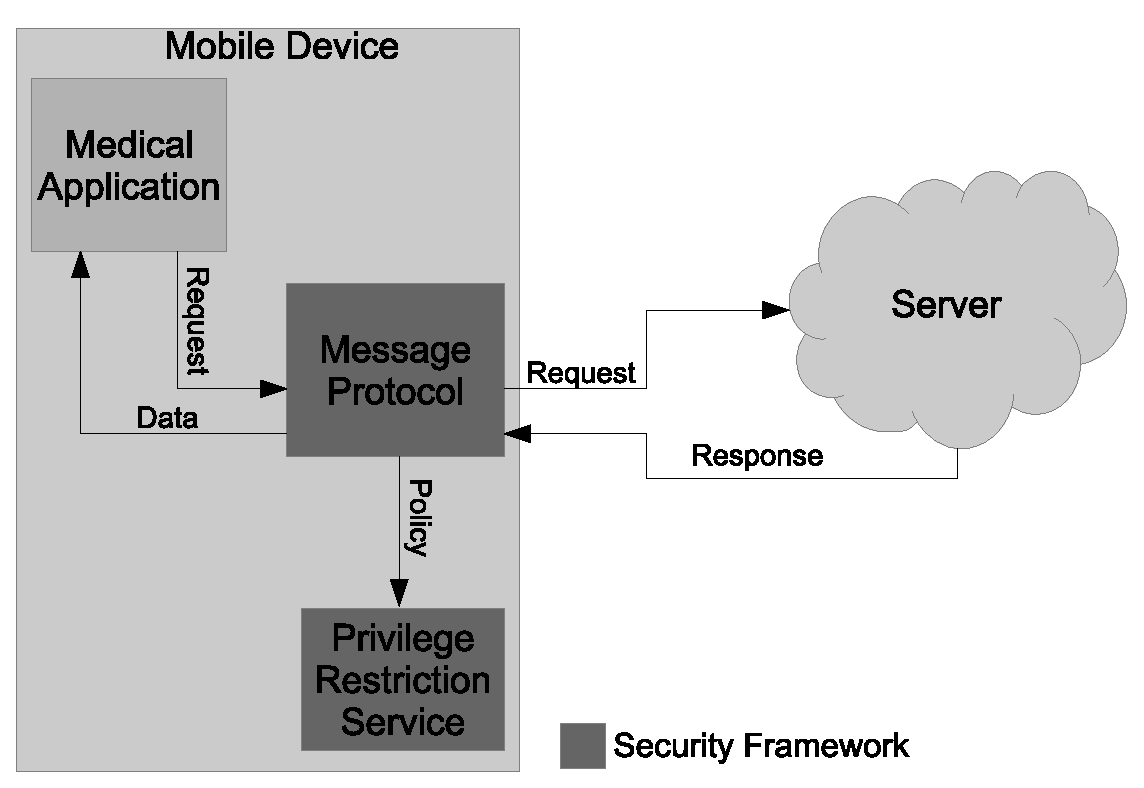
\psfig{file=frameworkcomponent.eps, width=2.5in}
\caption{Message Protocol Flow}
\label{fig:frameworkcomponents}
\end{figure}


